\section{Introduction}
\label{sec:intro}

Medical Large Vision-Language Models (Med-LVLMs) have shown impressive capabilities in medical VQA and report generation \cite{Li2023LLaVAMed, Moor2023MedFlamingo}. However, they often suffer from modality bias, relying on spurious background correlations rather than lesion evidence, leading to hallucinated outputs \cite{Royer2024MultiMedEval}.

\begin{figure}[!tbp]
    \centering
    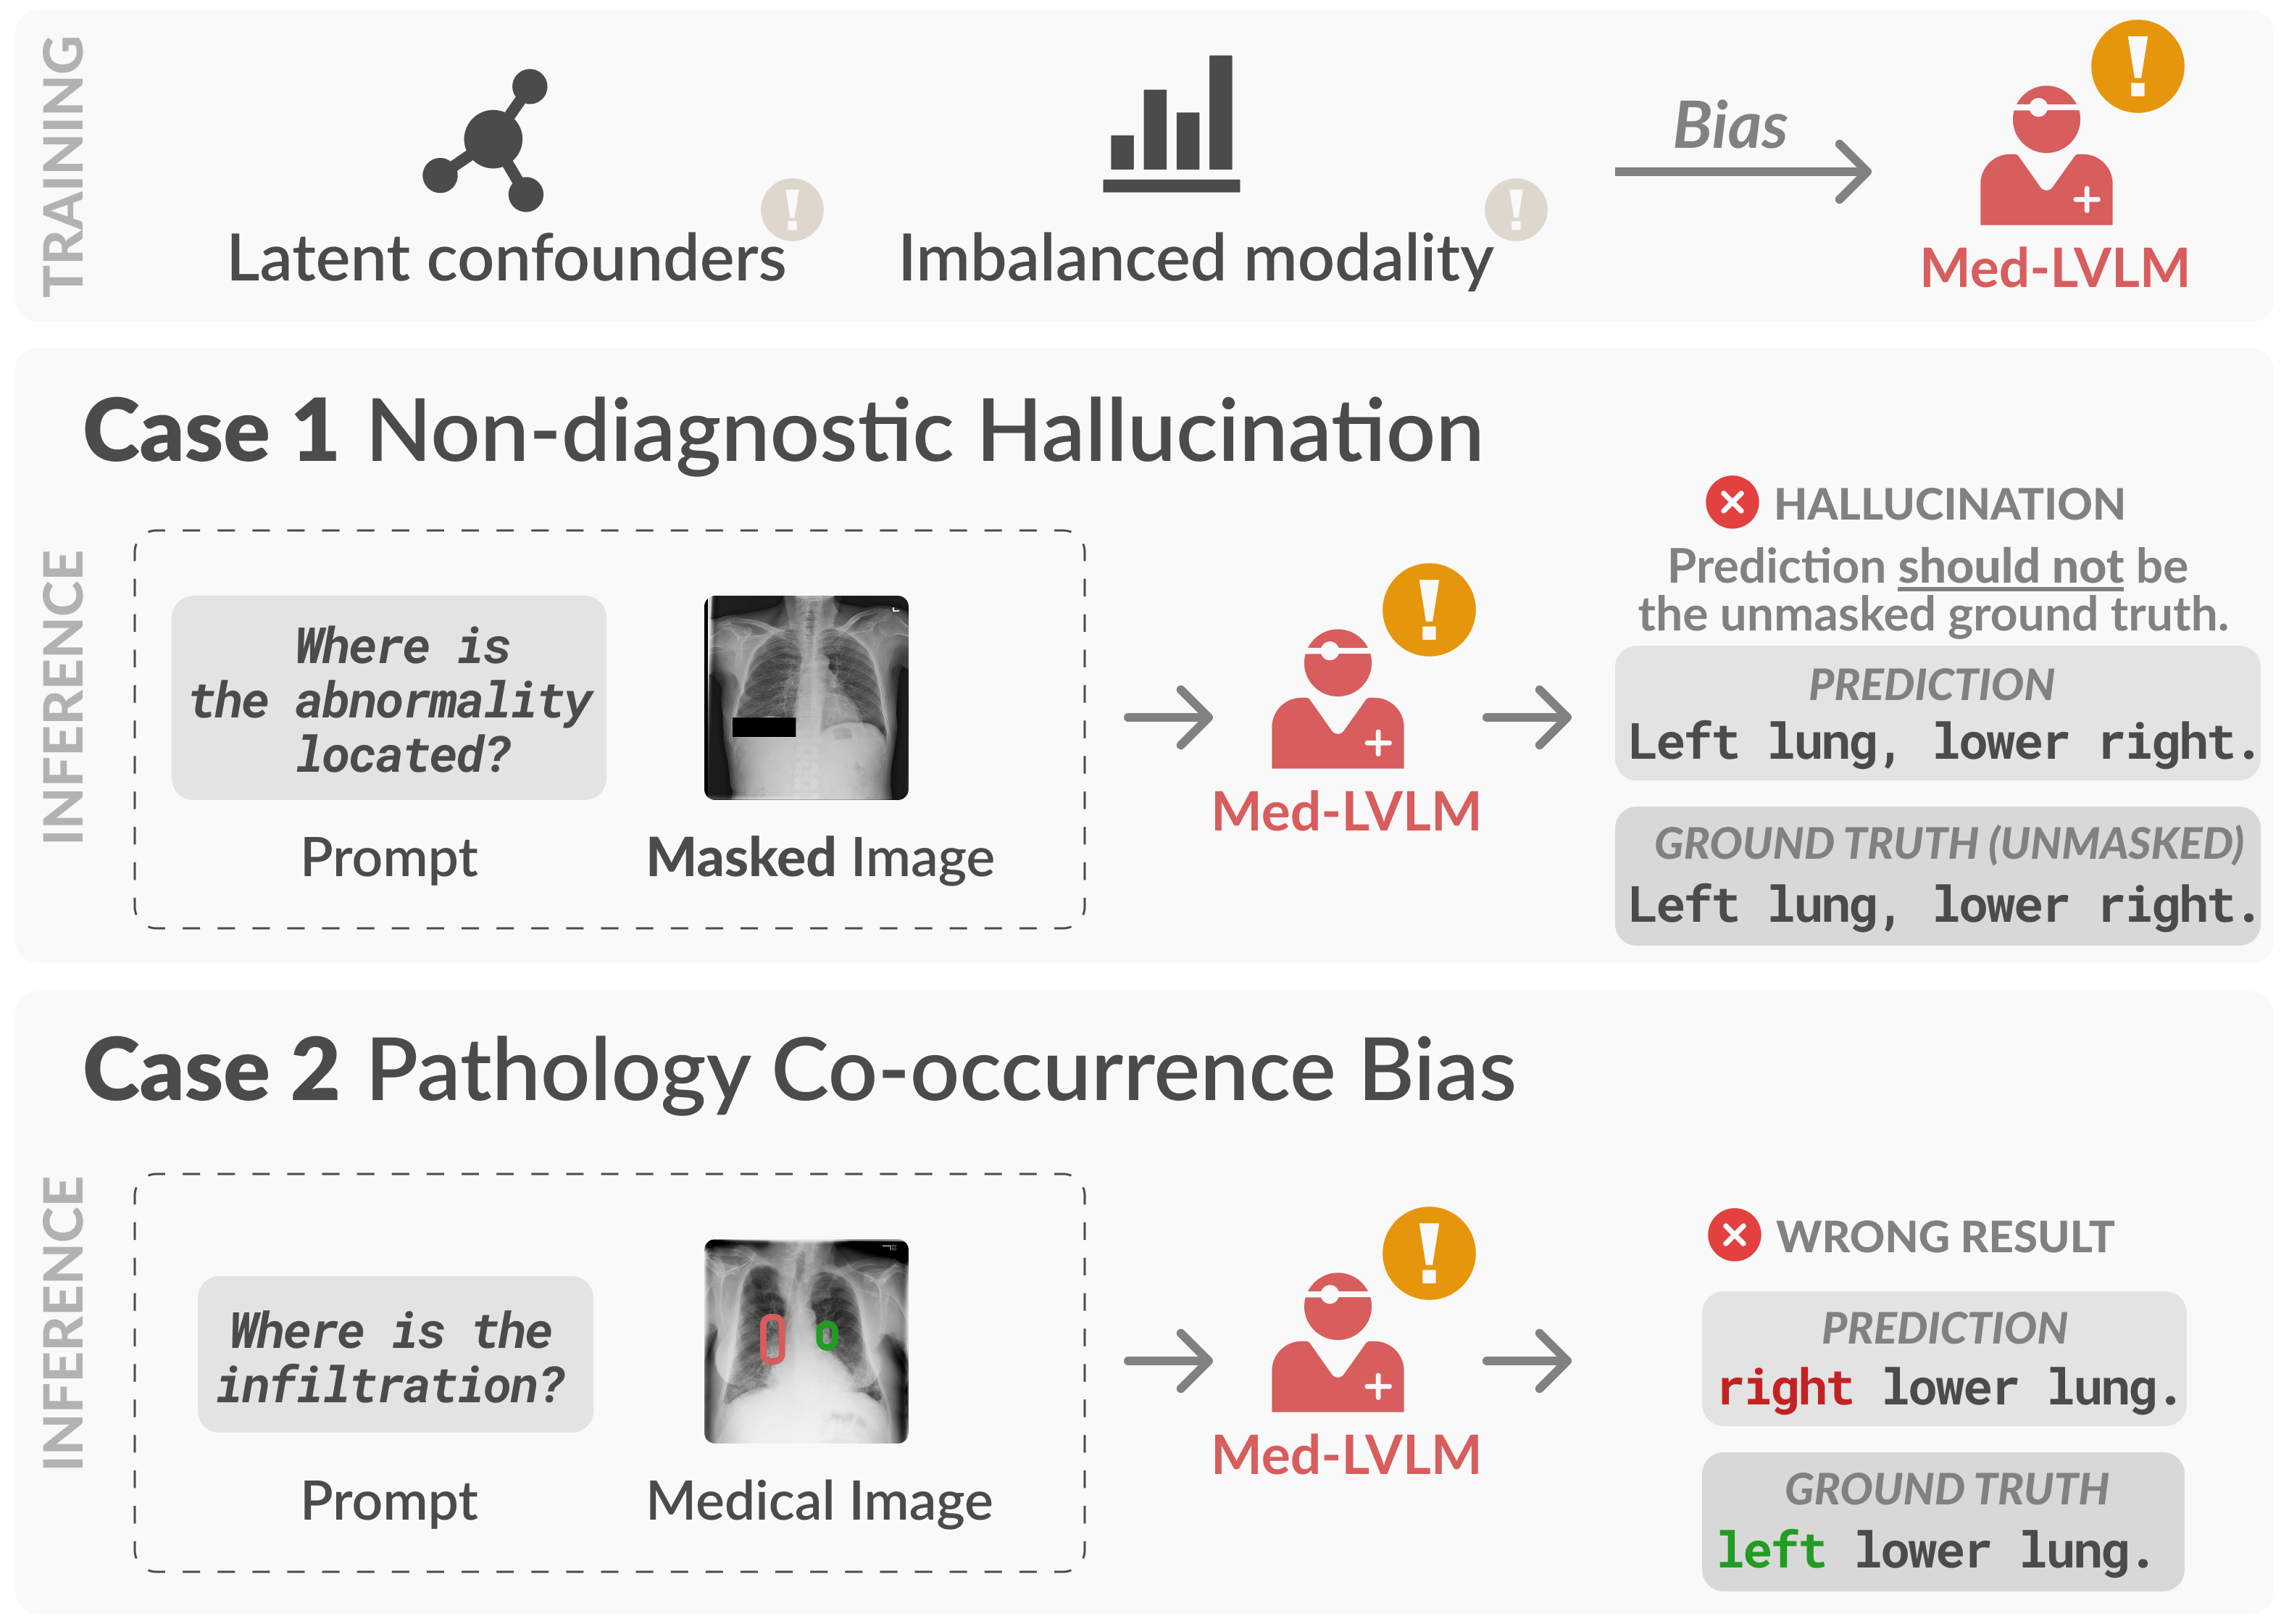
\includegraphics[width=0.5\textwidth]{figs/cvpr_fig1.png}
    \caption{Effects of spurious causation on inference.}
    \label{fig:intro}
    \vspace{-10pt}
\end{figure}

To address this, recent works introduce preference optimization \cite{rafailov2023direct, Zhu2025MMedPO}. However, they overlook spurious causation from biased modality interactions. We propose a \textbf{Ca}usal \textbf{Med}ical \textbf{P}reference \textbf{O}ptimization framework (\textbf{CaMedPO}) that mitigates spurious causation while preserving the valuable indirect effect between lesion and background.

Our main contributions are threefold:
$\bullet$ We introduce a causal framework analyzing how biased reference policies propagate harmful direct effects.
$\bullet$ We propose CaMedPO, a model-agnostic debiasing approach constructing factual-counterfactual outcome pairs based on lesion detection.
$\bullet$ Extensive experiments on Med-VQA and report generation benchmarks demonstrate consistent improvements in factual accuracy.